\documentclass[12pt, a4paper]{article}

% --- PACOTES FUNDAMENTAIS ---
\usepackage[utf8]{inputenc}
\usepackage[T1]{fontenc}
\usepackage[brazil]{babel}
\usepackage{helvet}
\renewcommand{\familydefault}{\sfdefault}
\usepackage{amsmath}
\usepackage{graphicx}
\usepackage{enumitem}
\usepackage{indentfirst}
\usepackage{setspace}
\usepackage{xurl}
\usepackage[hidelinks]{hyperref}
\urlstyle{same}

% --- CONFIGURAÇÃO DE MARGENS E CABEÇALHO ---
\usepackage[a4paper, top=4cm, headheight=2.5cm, bottom=2cm, left=3cm, right=2cm]{geometry}
\usepackage{fancyhdr}

\pagestyle{fancy}
\fancyhf{} 
\renewcommand{\headrulewidth}{0pt}
\chead{\noindent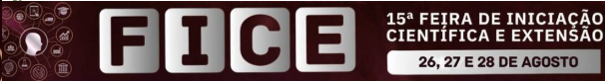
\includegraphics[width=\textwidth]{Imagem1.png}}

% --- ESPAÇAMENTO DAS NOTAS DE RODAPÉ ---
\setlength{\skip\footins}{1.5cm} 

% --- ATALHO DE FORMATAÇÃO DAS SEÇÕES ---
\newcommand{\titlesection}[1]{
    \vspace{1.5em}
    \noindent\textbf{\MakeUppercase{#1}}
    \vspace{1em}\par
}

\begin{document}
\onehalfspacing

% --- TÍTULO E AUTORES ---
\begin{center}
    \textbf{TÍTULO DO TRABALHO FINAL: Subtítulo (se houver)}
    
    \vspace{1.5em}
    Nome do Autor 1$^{1}$; Nome do Autor 2$^{2}$; Nome do Autor 3$^{3}$; Nome do Orientador$^{4}$
\end{center}

% Notas de rodapé com afiliações
\footnotetext[1]{Estudante do curso de Ciência da Computação. Instituto Federal Catarinense (IFC) - Campus Videira. E-mail: autor1@email.com}
\footnotetext[2]{Estudante do curso de Ciência da Computação. Instituto Federal Catarinense (IFC) - Campus Videira. E-mail: autor2@email.com}
\footnotetext[3]{Estudante do curso de Ciência da Computação. Instituto Federal Catarinense (IFC) - Campus Videira. E-mail: autor3@email.com}
\footnotetext[4]{Professor Orientador. Instituto Federal Catarinense (IFC) - Campus Videira. E-mail: orientador@ifc.edu.br}

% --- INTRODUÇÃO ---
\titlesection{INTRODUÇÃO}
[Insira aqui a introdução do relatório final. Lembre-se de utilizar os verbos no passado, pois o projeto já foi concluído (ex: "O objetivo geral deste trabalho foi...").]

% --- PROCEDIMENTOS METODOLÓGICOS ---
\titlesection{PROCEDIMENTOS METODOLÓGICOS (materiais e métodos)}

[Descreva como o projeto foi de fato executado:]

\begin{enumerate}[label=\alph*)]
    \item Início e término da implementação do projeto: [Ex: fevereiro a julho de 2026].
    \item Local onde foi desenvolvido o trabalho: Instituto Federal Catarinense (IFC) - Campus Videira.
    \item População envolvida: [Público-alvo atingido ou testado].
    \item Instrumentos utilizados: [Linguagens, frameworks, banco de dados, bibliotecas utilizadas].
    \item Procedimentos: [Arquitetura implementada e regras de negócio codificadas].
    \item Métodos de análise dos dados: [Testes realizados para validar o sistema].
\end{enumerate}

% --- RESULTADOS E DISCUSSÕES ---
\titlesection{RESULTADOS E DISCUSSÕES}
[Apresente aqui o que foi desenvolvido. Foque nas principais funcionalidades, na arquitetura do software criado, em métricas de desempenho (se houver) e na análise técnica do produto final. Imagens de protótipos de tela ou trechos críticos de lógica (como fórmulas matemáticas ou algoritmos de ranking) podem enriquecer esta seção.]

% --- CONSIDERAÇÕES FINAIS ---
\titlesection{CONSIDERAÇÕES FINAIS}
[Sintetize se os problemas propostos na introdução foram resolvidos pelo software construído. Apresente os aprendizados técnicos e mencione possíveis trabalhos futuros ou melhorias que podem ser feitas na aplicação em novas versões.]

% --- REFERÊNCIAS ---
\begin{center}
    \vspace{1.5em}
    \textbf{REFERÊNCIAS}
    \vspace{1em}
\end{center}

\begin{singlespace}
\noindent SOBRENOME, Nome do Autor. \textbf{Título do livro ou artigo em negrito}. Edição. Cidade: Editora, Ano.

\vspace{1em}
\noindent SOBRENOME, Nome do Autor 2. Título do artigo. \textbf{Nome da Revista em negrito}, Cidade, v. 1, n. 1, p. 1-10, Ano.
\end{singlespace}

\end{document}